\documentclass[aspectratio=169,xcolor=table]{beamer}
%aspcetratio >> 1610 169 149 54 43 32
%The themes:
%\usetheme[style=classic]{mharvellous}
\usetheme[style=dark]{mharvellous}
%\usetheme[style=mracula]{mharvellous}
%\usetheme[style=default]{mharvellous}
%*--------------------------------------------------
%\usepackage{helvet}
%*--------------------------------------------------
\usepackage{bibunits}  
%\setbeamertemplate{bibliography item}{[\theenumiv]}
\setbeamertemplate{bibliography item}{\insertbiblabel}
\defaultbibliography{bibliography}
%\defaultbibliographystyle{IEEEtran}
%\defaultbibliographystyle{amsalpha}
\defaultbibliographystyle{abntex2-alf}
%\bibliography{bibliography}
%\usepackage[backend=biber,style=alphabetic,citestyle=authoryear]{biblatex}
% \addbibresource{bibliography.bib}
%\usepackage{natbib}
\usepackage{bibentry}
%*--------------------------------------------------
\usepackage{lipsum}
\usepackage{epigraph}
\usepackage{graphicx}
\usepackage{multirow}
%\usepackage{enumitem}
\usepackage{array}
%\usepackage{multimedia}
\usepackage{media9}
%\usepackage{pdfpc-movie}
\usepackage{circledsteps}
\usepackage{listings}
\usepackage[normalem]{ulem}
%\usepackage{Sweave}
%\usepackage{xkeyval}
%\usepackage{palatino}
%\usepackage{pgfpages}
\usepackage{float}
%*--------------------------------------------------
\usepackage[timeinterval=1]{tdclock}
%\usepackage[font=Times,timeinterval=1, timeduration=200,resetatpages=all]{tdclock}
%\usepackage[font=Times,timeinterval=10, timeduration=2.0, timedeath=0, fillcolorwarningsecond=white!60!yellow,timewarningfirst=50,timewarningsecond=80,resetatpages=2]{tdclock}
%*--------------------------------------------------
\usepackage{url}
\usepackage{tabularx,booktabs}
\usepackage{threeparttable}
\usepackage[absolute, overlay]{textpos}
%*--------------------------------------------------
\usepackage{framed, color}
\usepackage[tikz]{bclogo}
\usepackage{spot}
\setspotlightcolor{red!50}
% %\setspotlightstyle{star, fill=red!50}
% %\setspotlightstyle{star points=7}
\usepackage{color,soul}
%\usepackage{xcolor}
\usepackage{tcolorbox}
\usepackage{xcolor}
\usepackage[export]{adjustbox}
\usepackage{verbatim}
\usetikzlibrary{trees,shapes,arrows}
\usepackage{fancyvrb}
\usepackage{float}
%*--------------------------------------------------
\usepackage{amsmath}
\usepackage{xfrac}
\usepackage{units}
\usepackage{ulem}
%*-------------------------------------------------------------------------------
%\newcolumntype{C}[1]{>{\centering\arraybackslash}m{#1}}
\newcolumntype{L}[1]{>{\raggedright\let\newline\\\arraybackslash\hspace{0pt}}m{#1}}
\newcolumntype{C}[1]{>{\centering\let\newline\\\arraybackslash\hspace{0pt}}m{#1}}
\newcolumntype{R}[1]{>{\raggedleft\let\newline\\\arraybackslash\hspace{0pt}}m{#1}}
%*-------------------------------------------------------------------------------
%\pgfpagesuselayout{2 on 1}[a4paper,border shrink=5mm]
%\setbeamertemplate{note page}[plain]
%\setbeameroption{show notes on second screen=bottom}
%*-------------------------------------------------------------------------------
\setbeameroption{hide notes}
%\setbeameroption{show only notes}
%\setbeameroption{show notes on second screen=right}
\setbeamertemplate{note page}{\pagecolor{yellow!5}\insertnote}
%*-------------------------------------------------------------------------------

%*-------------------------------------------------------------------------------
\title              {P-OO-ng}
\subtitle           {Plataforma de jogo em Processing com Arduino integrado}
\author             {Ludmila Nascimento, Rafael Mello, Kauan Dantas e Gabriel Lopes}
\advisor            {Orientador: Marco A. dos Reis}
\institute          {Robótica e Sistemas Autônomos, Senai Cimatec}
\date               {Julho de 2022}
% \ulogo        		{Template/logosenaicimatecnegativo}
% \ulogof             {Template/logosenaicimatec2020}
% \ulogoo        		{Template/rosa-logo}
% \ulistelement    	{Template/bullet-white}

%*-------------------------------------------------------------------------------
\graphicspath{{Source/pictures/}}
%*-------------------------------------------------------------------------------
\totalNoSlidesDisabled % To turn off the total number of slides in the footer. Comment this if you want the total number of slides in the footer
%*-------------------------------------------------------------------------------
\begin{document}
%*----------- COVER -------------------------------------------------------------
 \begin{frame}[t,plain]
%*----------- sound--------------------------------
    \includemedia[
        %width=1ex,
        %height=1ex,
        %activate=pageopen, 
        activate=onclick,
        deactivate=onclick,
        %passcontext,
        transparent,
        addresource=./Source/sounds/hip-hop.mp3,
        flashvars={
                    source=./Source/sounds/hip-hop.mp3
                    %&autoPlay=true
                    &autoRewind=true
                    &Play=2s
                    &repeat=always
                    %&Loop=true
        }
    ]
    {}{VPlayer.swf}
%*----------- start-page--------------------------
    \titlepage
    %*----------- notes-------------------------------
    \note[item]{Notes can help you to remember important information. Turn on the notes option.}
\end{frame}
%-
%*----------- SECTIONS ----------------------------------------------------------
\section{Introdução}

Em 1972, na garagem de um grupo de engenheiros que criariam uma empresa de jogos futuramente, a Atari, surgiu, de um pequeno exercício de simulação o que muitos consideram como o primeiro jogo da história: o "Pong". Na tentativa de simular uma partida de tênis de mesa ou "Ping-Pong" como é conhecido, o jogo eletrônico foi incrementado pelo grupo que tornou o jogo mais divertido e apropriado para o público.

	Apesar de ter sido recusado por um cliente, alegando que prefereria um jogo de carros, um dos criadores não desistiu. "Bushnell convenceu um bar, chamado Andy Capp's, em Sunnyvale, na Califórnia, a instalar o Pong em uma máquina de fliperama —daquelas que funcionam com a inserção de moedas" (UOL, 2022). 

	Esse foi o salto inicial que, não só impulsionou o sucesso do jogo "Pong", mas também do mundo dos fliperamas, que teve sua alta na década de 80.

	Com isso em mente, o presente trabalho tem como finalidade de recriar o jogo "Pong" utilizando de tecnologias mais modernas. Em suma, através da integração de um Arduino UNO, que irá receber a informação dos botões e joysticks(potênciometros) e enviará por comunicação serial ao jogo, desenvolvido utilizando a linguagem de programação Open Source "Processing", utilizada para programação dentro do contexto de artes visuais[2].


%*----------- SLIDE -------------------------------------------------------------
\begin{frame}[c]{Processing}
    %\transboxin[duration=1,direction=30]
 
    \begin{itemize}
        \item Processing é uma linguagem de programação Open-Source e IDE (Ambiente de Desenvolvimento Integrado) construído para projetos visuais principalmente, e para servir como base de cadernos eletrônicos.
        \item É uma linguagem com grande assimilação às linguagens "C" e "Java", grandes inspirações da liguagem, resultando em algo que remete à programação em C com aspectos da programação orientada a objetos do Java.
    \end{itemize}
	\vspace{0.4cm}
	\centering
	
\includegraphics[width=0.3\textwidth]{processing-logo}   

%*----------- notes
    \note[item]{Notes can help you to remember important information. Turn on the notes option.}
\end{frame}
%-
%*----------- SLIDE -------------------------------------------------------------
\begin{frame}[t]{Arduino}
      \begin{itemize}
        \item Arduino é uma plataforma de prototipagem e hardware livre, projetado como um microcontrolador.
        \item Utilizando a liguagem C/C++ como base, o Arduino tornou-se bastante popular por apresentar baixo custo, flexibilidade e facilidade de manuseio em desenvolvimento de sistemas interativos.
    \end{itemize}
\vspace{0.3cm}
\begin{columns}
	% Column 1
	\begin{column}{0.4\textwidth}
        	\centering
		
\includegraphics[width=0.5\textwidth]{arduino-logo} 
	\end{column}
	% Column 2    
		\begin{column}{0.4\textwidth}
		\centering
       	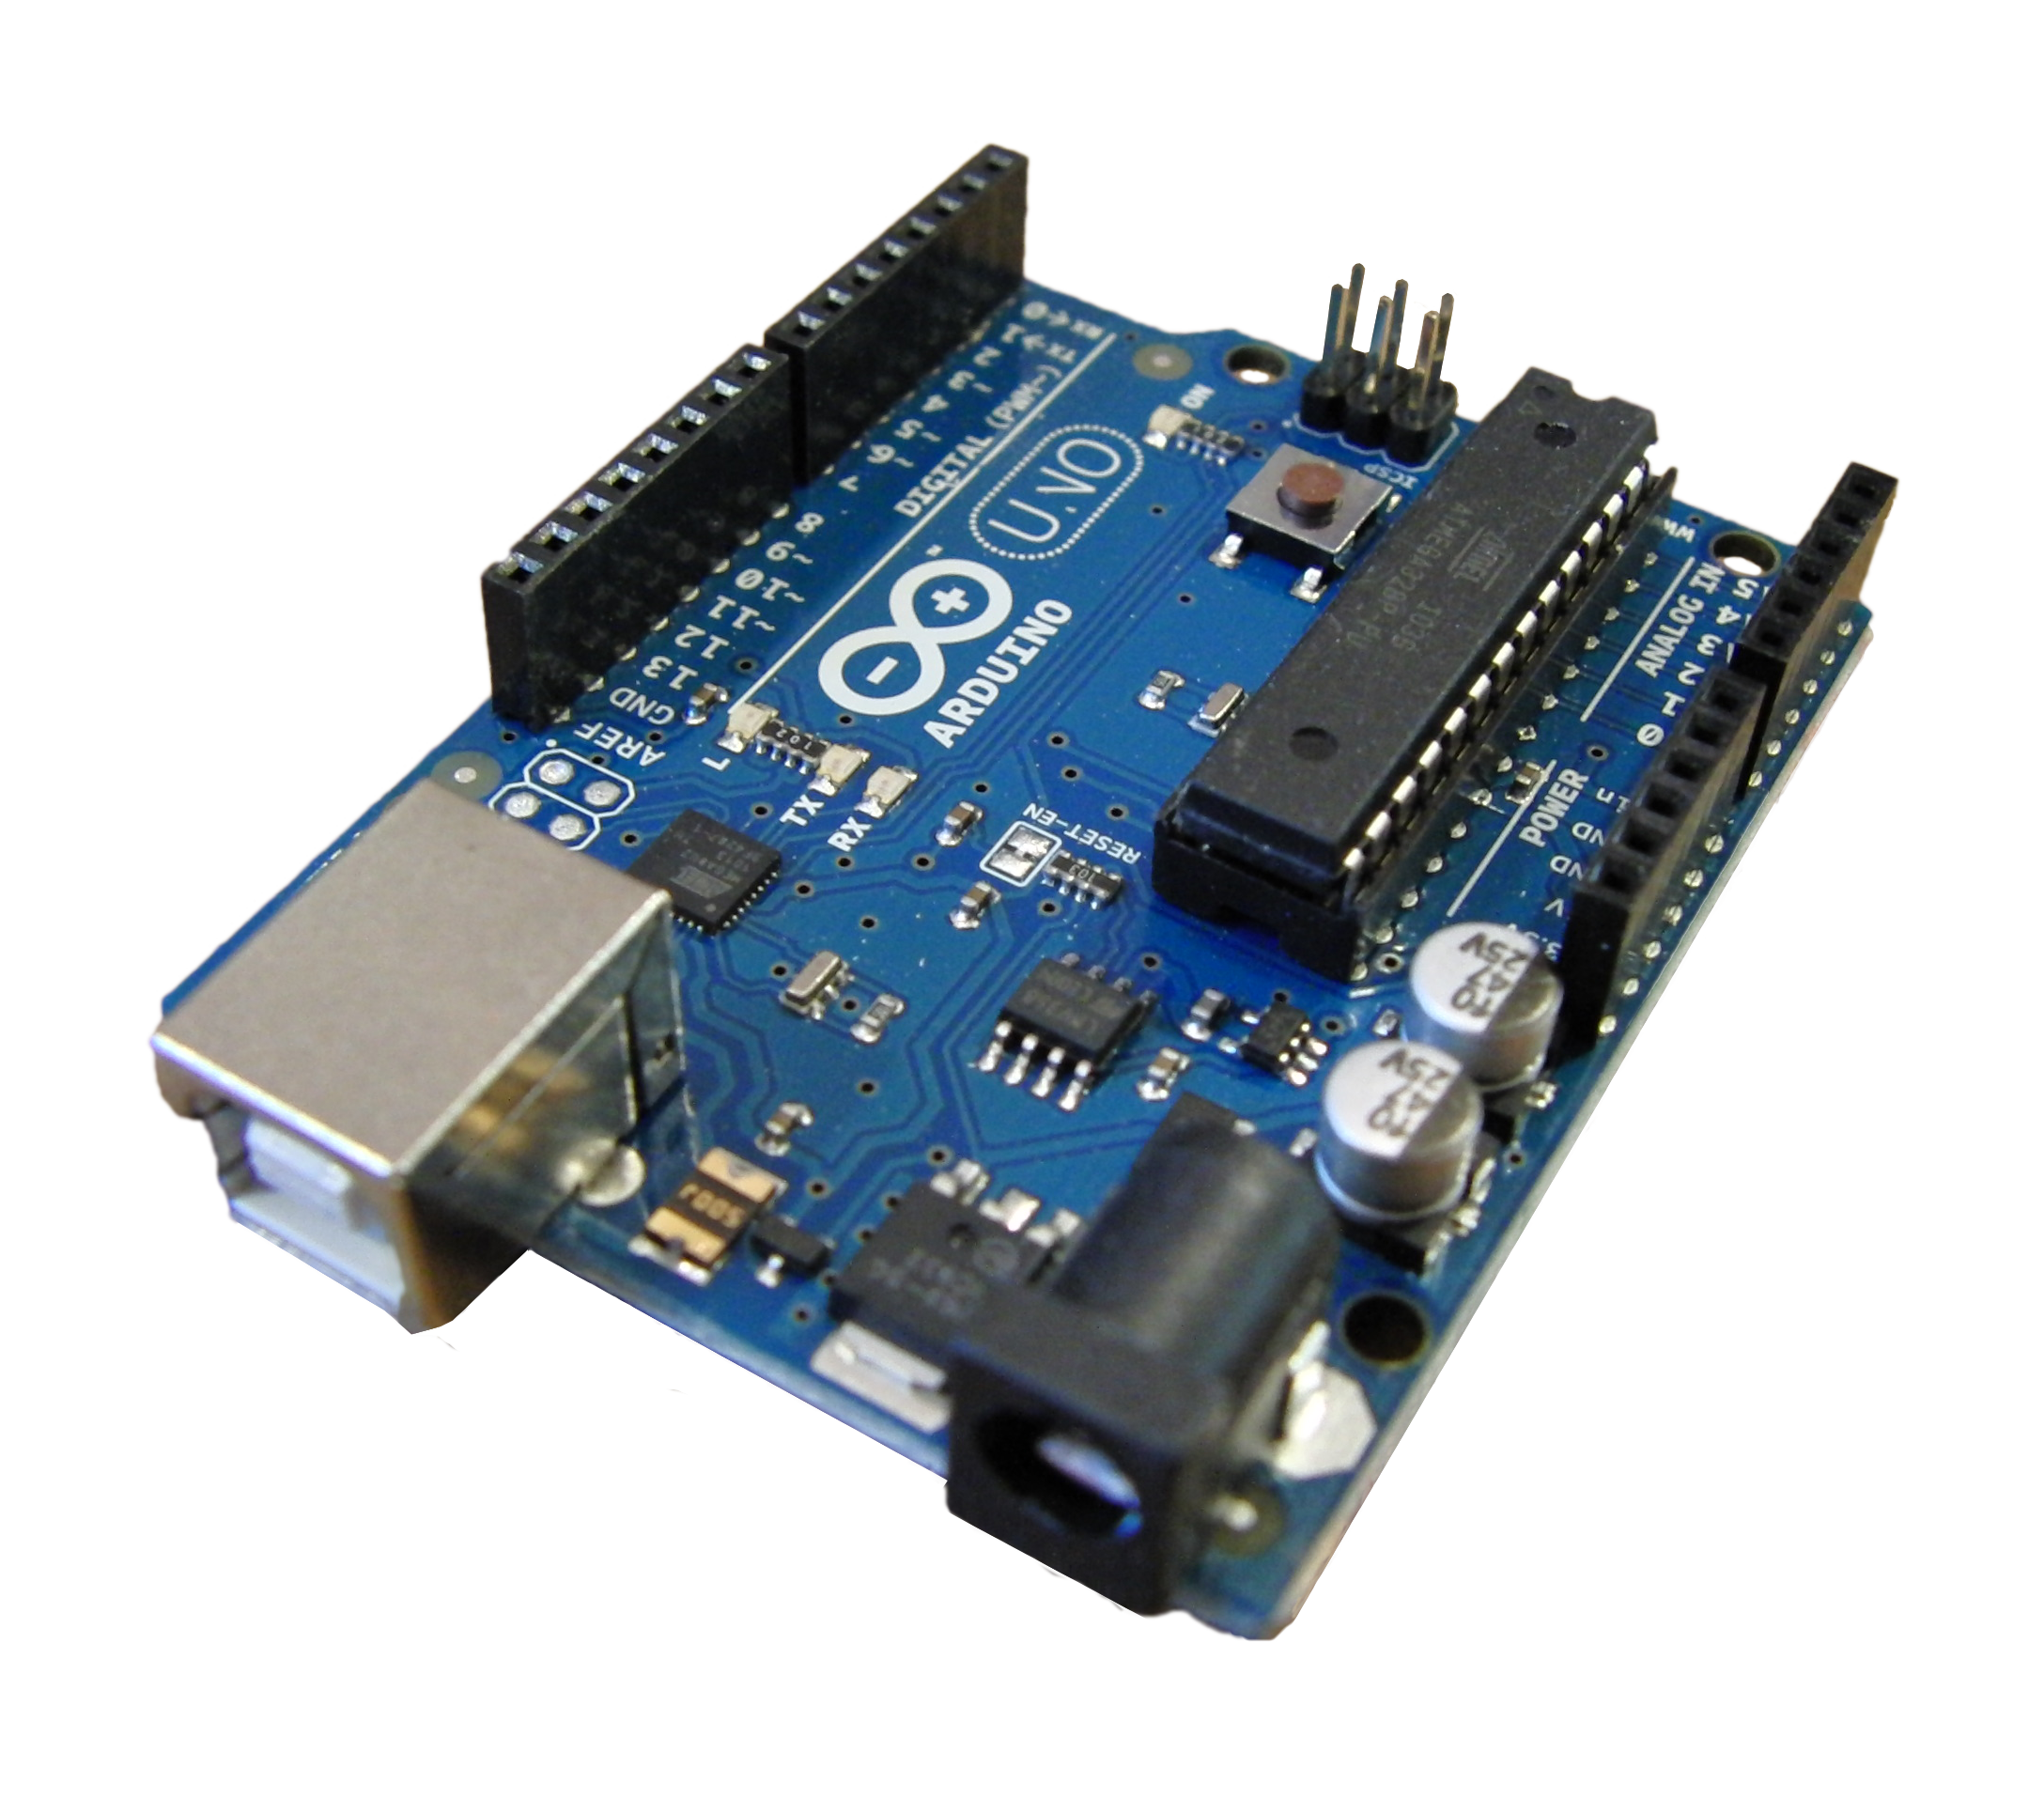
\includegraphics[width=0.7\textwidth]{arduino} 
	\end{column}
\end{columns}


%*----------- notes
    \note[item]{Notes can help you to remember important information. Turn on the notes option.}
\end{frame}

%*----------- SLIDE -------------------------------------------------------------
\begin{frame}[t]{As lideranças das equipes dos Novos Talentos}
    \vspace{0.5cm}
    \begin{columns}
        \column{.01\textwidth}
        \column{.7\textwidth}
            \begin{itemize}
                \item equipe \tikznode{cmark}{RAJA} será liderada por Aziel Freitas
                \item equipe \Circled[outer color=mracula8, inner ysep=8pt]{BORG} será liderada por Mateus Cerqueira.
                \item equipe \Circled[outer color=mracula7, inner ysep=8pt]{BORG} será liderada por Mateus Cerqueira.
                \item equipe \Circled[outer color=mracula9, inner ysep=8pt]{jerotimon} será liderada por Mateus Cerqueira.
                \item equipe TIMON-HM será liderada por Leonardo Lima.
            \end{itemize}
        \column{.29\textwidth}
            
\includegraphics[width=.9\textwidth, trim={10cm 0 10cm 0},clip]{equipe}
    \end{columns}
    \vspace{1cm}
    
    \emph{Para este desafio não será cobrado o relatório técnico, porém o acompanhamento deverá seguir o mesmo ritmo dos desafios anteriores.}

    %add circle on word
    \begin{tikzpicture}[remember picture,overlay]
        \draw[mracula5,very thick] (cmark) circle[x radius=8mm,y radius=4mm]; 
    \end{tikzpicture}
%*----------- notes
    \note[item]{Notes can help you to remember important information. Turn on the notes option.}
\end{frame}
%-
%*----------- SLIDE -------------------------------------------------------------
\begin{frame}[t]{O progresso das equipes}
    Um dos indicadores para o acompanhamento das equipes será o percentual de conclusão geral da equipe.
    O planejamento das atividades deverá seguir a metodologia aplicada no desenvolvimento de projetos de robótica.
    \newline
    %\vspace{0.5cm}
    \begin{table}[ht!]
    \centering
        \caption{PERCENTUAL DE CONCLUSÃO POR EQUIPE}
        \begin{tabular}{|l|c|c|c|c|} \hline
            \textbf{EQUIPE}&\textbf{04/05}&\textbf{11/05}&\textbf{18/05}&\textbf{25/05}\\ \hline
            RAJA & 17\% &32\% & &  \\ \hline
            BORG & 0\% &41\% & &  \\ \hline
            TIMON-HM & 5\% &47\% & &  \\ \hline
        \end{tabular}
    \end{table}
%*----------- notes
    \note[item]{Notes can help you to remember important information. Turn on the notes option.}
\end{frame}
%-
%*----------- SLIDE -------------------------------------------------------------
\begin{frame}[t]{O progresso das equipes}
    Um dos indicadores para o acompanhamento das equipes será o percentual de conclusão geral da equipe.
    O planejamento das atividades deverá seguir a metodologia aplicada no desenvolvimento de projetos de robótica.
    \newline
    %\vspace{0.5cm}
    % \begin{table}[ht!]
    % \centering
    %     \caption{PERCENTUAL DE CONCLUSÃO POR EQUIPE}
    %     \begin{tabular}{|l|c|c|c|c|} \hline
    %         \textbf{EQUIPE}&\textbf{04/05}&\textbf{11/05}&\textbf{18/05}&\textbf{25/05}\\ \hline
    %         RAJA & 17\% &32\% & &  \\ \hline
    %         BORG & 0\% &41\% & &  \\ \hline
    %         TIMON-HM & 5\% &47\% & &  \\ \hline
    %     \end{tabular}
    % \end{table}
%*----------- notes
    \note[item]{Notes can help you to remember important information. Turn on the notes option.}
\end{frame}
%-
%*----------- SLIDE -------------------------------------------------------------
\begin{frame}[t]{O progresso das equipes}
    Um dos indicadores para o acompanhamento das equipes será o percentual de conclusão geral da equipe.
    O planejamento das atividades deverá seguir a metodologia aplicada no desenvolvimento de projetos de robótica.
    \newline
    %\vspace{0.5cm}
    % \begin{table}[ht!]
    % \centering
    %     \caption{PERCENTUAL DE CONCLUSÃO POR EQUIPE}
    %     \begin{tabular}{|l|c|c|c|c|} \hline
    %         \textbf{EQUIPE}&\textbf{04/05}&\textbf{11/05}&\textbf{18/05}&\textbf{25/05}\\ \hline
    %         RAJA & 17\% &32\% & &  \\ \hline
    %         BORG & 0\% &41\% & &  \\ \hline
    %         TIMON-HM & 5\% &47\% & &  \\ \hline
    %     \end{tabular}
    % \end{table}
    
    \url{https://braziliansinrobotics.com/}
%*----------- notes
    \note[item]{Notes can help you to remember important information. Turn on the notes option.}
\end{frame}
%-
%*----------- SLIDE -------------------------------------------------------------
\begin{frame}[t]{Hardware}

	\begin{itemize}
        \item Circuito utilizado como os controles do jogo
	\item Os potenciômetros controlam as barras (paddles)
	\item Os botões fazem a transição de telas e pausam o jogo.
    \end{itemize}
   
	\vspace{0.3cm}
	\begin{columns}
		% Column 1
		\begin{column}{0.5\textwidth}
			\begin{figure}
				\centering
					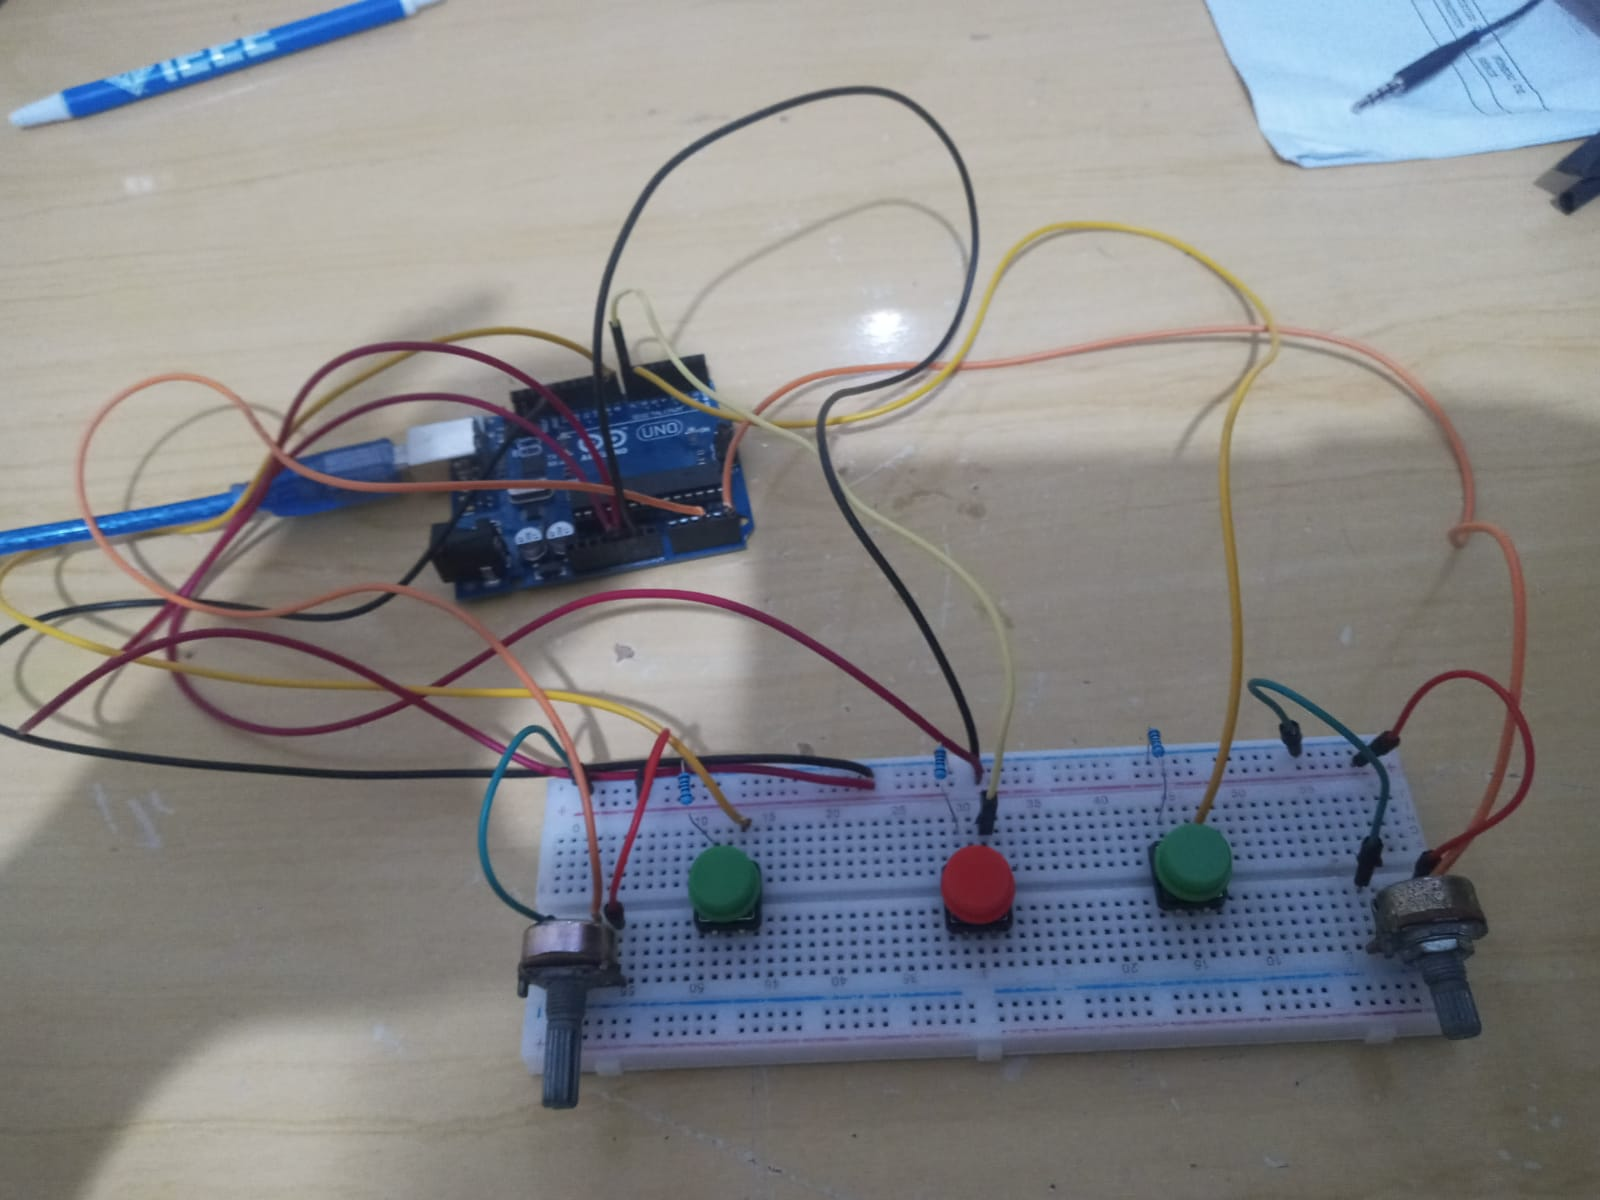
\includegraphics[width=0.6\textwidth]{circuito}
			\end{figure}
		\end{column}
			% Column 2    
			\begin{column}{0.7\textwidth}
				\begin{figure}
					\centering
						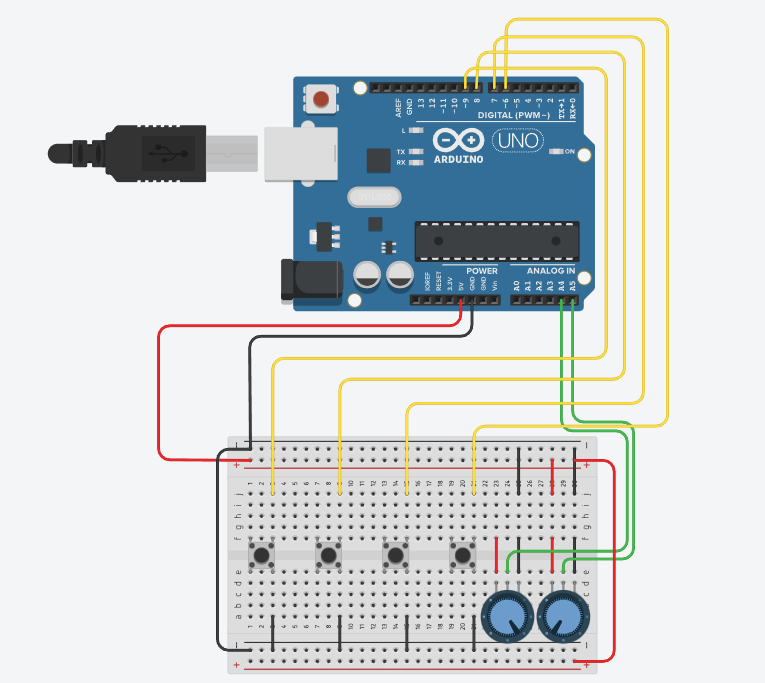
\includegraphics[width=0.4\textwidth]{esquematico-arduino}
				\end{figure}
			\end{column}
		\end{columns}

%*----------- notes
    \note[item]{Notes can help you to remember important information. Turn on the notes option.}
\end{frame}
%-
%*----------- SLIDE -------------------------------------------------------------
\begin{frame}[c]{Hardware - Controles}
 
  \begin{itemize}
      \item Modelos Impressos 3D para acomodar os botões e potenciômetros do circuito.
	\item Estes também são mais cômodos para os jogadores
    \end{itemize}
\vspace{0.3cm}
\begin{columns}
	% Column 1
	\begin{column}{0.4\textwidth}
		\begin{figure}
			\centering
    			\includegraphics[width=0.6\textwidth]{botão}
    			\caption{Os modelos impressos.}
    			%%\label{fig:question}
		\end{figure}
	\end{column}
		% Column 2    
		\begin{column}{0.4\textwidth}
			\begin{figure}
				\centering
    				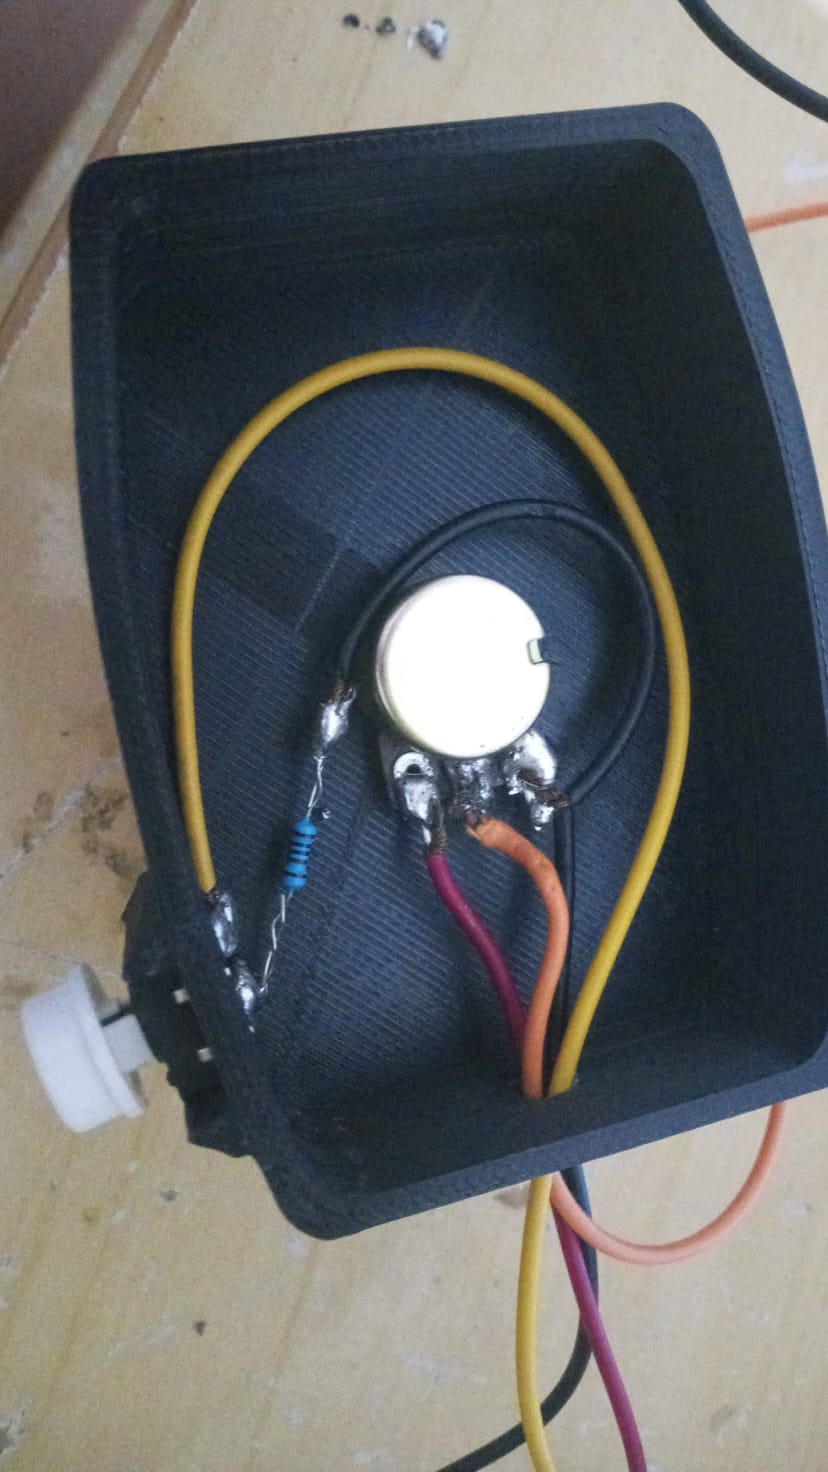
\includegraphics[width=0.4\textwidth]{solda}
    				\caption{A solda cos componentes no controle.}
    				%%\label{fig:question}
			\end{figure}
		\end{column}
	\end{columns}
%*----------- notes
    \note[item]{Notes can help you to remember important information. Turn on the notes option.}
 \end{frame}
%-
%*----------- SLIDE -------------------------------------------------------------
\begin{frame}[fragile]{Hardware - Arduino}
	 
\scriptsize
\begin{columns}
% Column 1
\begin{column}{0.5\textwidth}
	\begin{lstlisting}[language=C]
const int pot1 = A0, pot2 = A1; 
const int b01 = 8, b02 = 7; 
int v_pot1 = 0, v_pot2 = 0; 
bool v_b01,v_b02; 
int arr[10];

void setup() {
	Serial.begin(9600);
	pinMode(pot1, INPUT);
	pinMode(pot2, INPUT);
	for(int i = 7; i <= 8; i++){
	pinMode(i, INPUT_PULLUP);
	}
}
	\end{lstlisting}
\end{column}
% Column 2    
\begin{column}{0.55\textwidth}
	\begin{lstlisting}[language=C]
void loop() {

v_pot1 = map(analogRead(pot1),0,1023,0,255);
Serial.print(String(v_pot1) + "-");

v_pot2 = map(analogRead(pot2),0,1023,0,255);
Serial.print(String(v_pot2) + "-");

v_b01 = !digitalRead(b01);
v_b02 = !digitalRead(b02);

Serial.print(String(v_b01) + "-");
Serial.print(String(v_b02) + "\n");
delay(50);

}		
	\end{lstlisting}
\end{column}
\end{columns} 


%*----------- notes
    \note[item]{Notes can help you to remember important information. Turn on the notes option.}
 \end{frame}
%-
%*----------- SLIDE -------------------------------------------------------------
\begin{frame}[c]{Hardware - Arduino}
\vspace{0.2cm}
\begin{itemize}
        \item Como pode ser visto, uma string de modelo [x-x-x-x] é enviada ao Processing serialmente.
	  \item No Processing, essa string será separada em caracteres e cada um sera atribuido a sua respectiva classe.
    \end{itemize}

\begin{figure}
	\centering
    	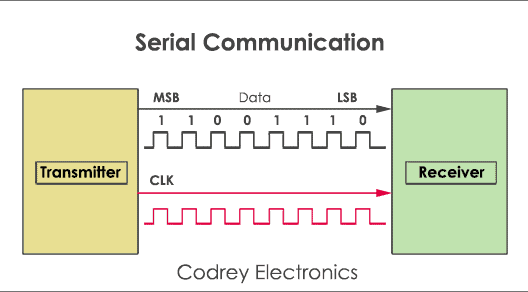
\includegraphics[width=0.4\textwidth]{serial}
    	%\caption{Representação d}
    	%%\label{fig:question}
\end{figure}

%*----------- notes
    \note[item]{Notes can help you to remember important information. Turn on the notes option.}
 \end{frame}
 %-
%*----------- SLIDE -------------------------------------------------------------
\begin{frame}
    

    
%*----------- notes
    \note[item]{Notes can help you to remember important information. Turn on the notes option.}
 \end{frame}
 %-
%*----------- SLIDE -------------------------------------------------------------
\begin{frame}
    %\transdissolve[duration=0.5]
    %\hspace*{-1cm}

  
 %*----------- notes__
    \note[item]{Notes can help you to remember important information. Turn on the notes option.}
\end{frame}
%-
%*----------- SLIDE -------------------------------------------------------------
\begin{frame}
    
  
 %*----------- notes__
    \note[item]{Notes can help you to remember important information. Turn on the notes option.}
\end{frame}
%-
%*----------- SLIDE -------------------------------------------------------------
\begin{frame}
    %\transdissolve[duration=0.5]
    
  
 %*----------- notes__
    \note[item]{Notes can help you to remember important information. Turn on the notes option.}
\end{frame}
%-
%*----------- SLIDE -------------------------------------------------------------
\begin{frame}
    %\transdissolve[duration=0.5]
    %\hspace*{-1cm}

  
 %*----------- notes
    \note[item]{Notes can help you to remember important information. Turn on the notes option.}
\end{frame}
 %-
%*----------- SLIDE -------------------------------------------------------------
\begin{frame}
    %\transdissolve[duration=0.5]
    %\hspace*{-1cm}
    
  
 %*----------- notes
    \note[item]{Notes can help you to remember important information. Turn on the notes option.}
\end{frame}
%-


%----------------------------------------------------SLIDE------------------
 \begin{frame}[t, allowframebreaks]{References}
 %\frametitle{References}
%\begin{frame}{Reference}
    %\transboxin[duration=1,direction=30]

    % \begin{bibunit}[plain]
    % \cite{guangyi2018research}.
    % %\cite{kanakia2012}
    % %\cite{agostini2007}
    % %\cite{azuma1997survey}
    % \cite{Buss2005}
  
    % \putbib
    % \end{bibunit}
  
    %\bibliographystyle{IEEEtran}
    %\bibliographystyle{IEEEtranS}
    %\bibliographystyle{IEEEbib}
    \bibliographystyle{abntex2-alf}
    %\bibliographystyle{abntex2-num}
    %\bibliographystyle{abnt-alf}
    \bibliography{bibliography} 
    %\putbib

%*----------- notes
    %\note[item]{Notes can help you to remember important information. Turn on the notes option.}
\end{frame}
%
%-
%*----------- SLIDE-BACKUP ------------------------------------------------------
% \backupbegin
% %
% \begin{frame}{Backup}
%     Test
% %*----------- notes-------------------------------
% \note{Notes can help you to remember important information. Turn on the notes option.}
% \end{frame}
% %-
% \backupend
% %-
%*----------- QUESTIONS ---------------------------------------------------------
\begin{frame}[c,plain]
    \lastpage{
        \begin{center}   
            {\usebeamerfont{title} Questions?}\\[3ex] 
            %\hspace{1.5cm} 
            marco.a.reis@google.com
        \end{center}
    }
    
    %*----------- notes---------------------------------
    \note[item]{Notes can help you to remember important information. Turn on the notes option.}
\end{frame}
%*-------------------------------------------------------------------------------
\end{document}